\subsection{Lab12: Retransmisión emisora mp3 online en FM estéreo}

%*********************
\begin{frame}{}

\pgfdeclareimage[width=\paperwidth,height=\paperheight]{bg}{imagenes/fondo_lab}
\setbeamertemplate{background}{\pgfuseimage{bg}}

\bfseries{\textrm{\LARGE Lab12\\ \Large Retransmisión emisora mp3 \newline online en FM estéreo}}
\raggedright
\end{frame}
%*********************

\begin{frame}{Introducción}

\pgfdeclareimage[width=\paperwidth,height=\paperheight]{bg}{imagenes/fondo3}
\setbeamertemplate{background}{\pgfuseimage{bg}}

Se realizará la retransmisión de una emisora online utilizando el transmisor de FM estéreo construido en la práctica anterior; se aprovechará  la característica de un archivo “ducto” o “tubería”, el cual nos permite que procesos separados se comuniquen sin haber sido diseñados para funcionar juntos. Gracias a la herramienta \texttt{mpg123} que lee uno o más archivos de audio o en este caso una URL que contiene un flujo de bits de audio en formato MPEG, es posible alimentar un archivo FIFO que se comporta como tubería; es decir en la medida que ingresan los bits de información de la emisora online en la “tubería”, así mismo son extraídos por el transmisor de radio FM estéreo y son retransmitidos.\cite{linuxjournal1995}.

\end{frame}
%---------------------------------

\begin{frame}{Esquema general}
    
\begin{figure}[H]
\centering
\vspace{-3mm}
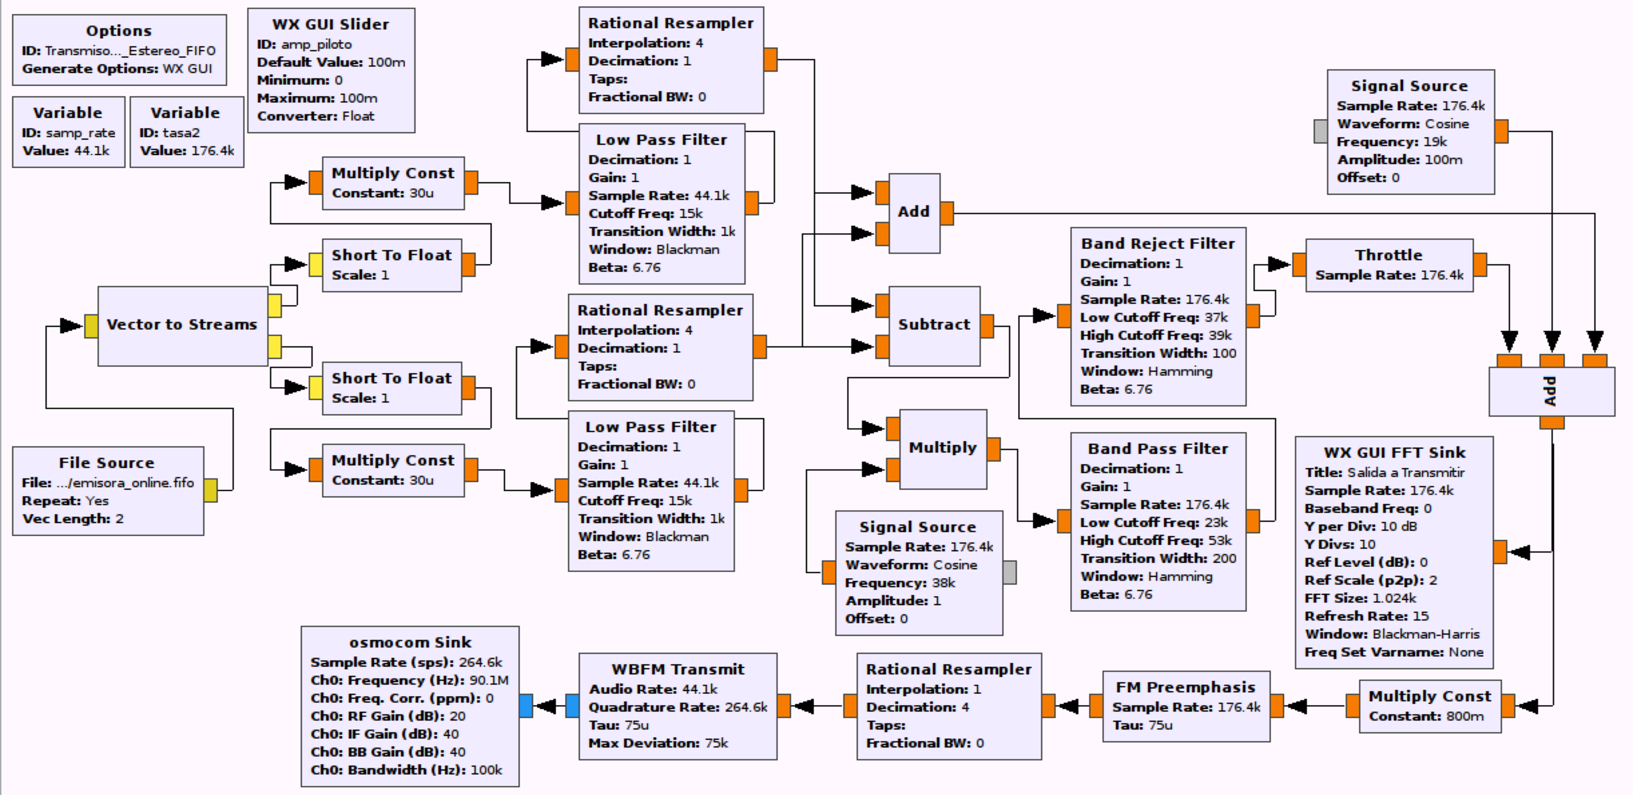
\includegraphics[width=\textwidth]{parte3/lab13/pdf/lab13_1.pdf}
\end{figure}
    
\end{frame}
%---------------------------------

\begin{frame}{Obtención URL emisora online}
    
\begin{figure}[H]
\centering
\vspace{-3mm}
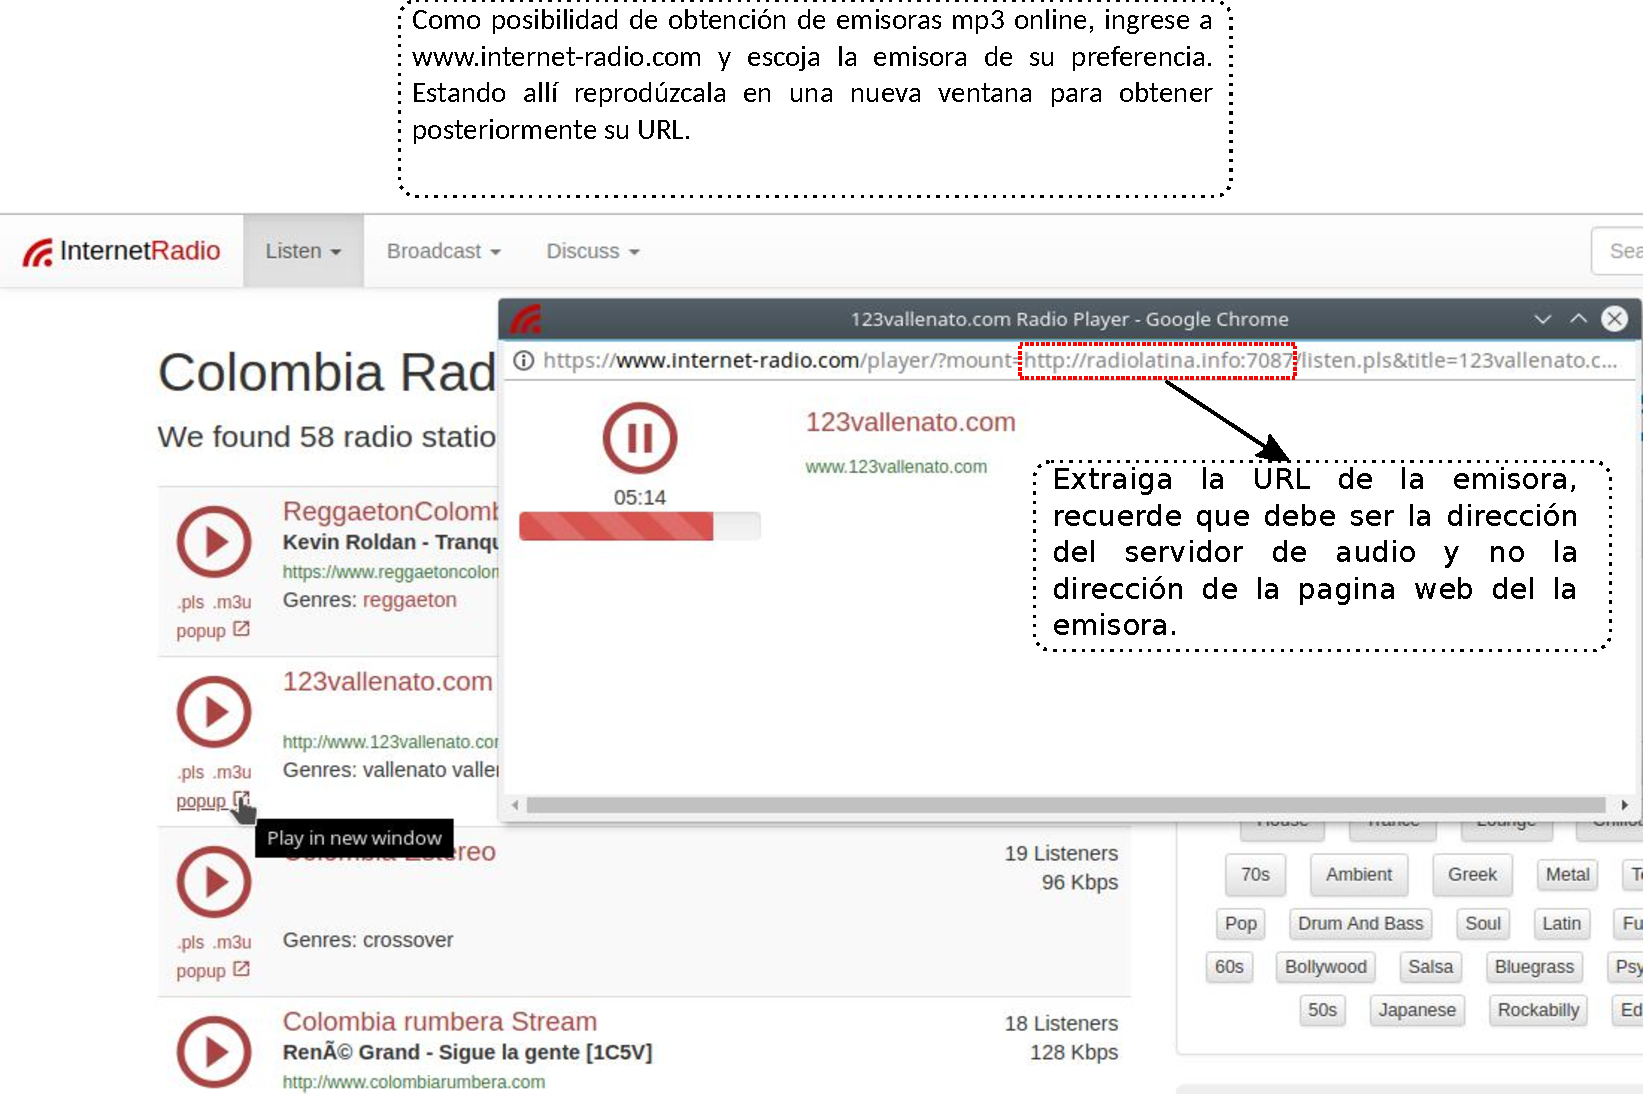
\includegraphics[width=.9\textwidth]{parte3/lab13/pdf/lab13_2.pdf}
\end{figure}
    
\end{frame}
%---------------------------------

\begin{frame}{Creación archivo FIFO}

Existe un tipo de tubería que puede ser descrita como una tubería “con nombre”, también denominada FIFO que sus siglas traducen “Primero en entrar, primero en salir” y se refiere a la propiedad de que el orden de bytes entrante es el mismo que sale.

\begin{itemize}
    \item {Mediante el uso de consola procedemos a introducir el comando mkfifo, que nos permite crear el archivo FIFO.
    
    \begin{block}{}
    \texttt{
    \ \ \ mkfifo emisora\_online.fifo}
    \end{block}
    }
    \item {Mediante la herramienta \texttt{mpg123} se procede a alimentar el archivo FIFO con una emisora online.
    
    \begin{block}{}
    \texttt{
    \ \ \ mpg123 -r44100 --stereo -s http://radiolatina.info:7087>emisora\_online.fifo}
    \end{block}
    }
\end{itemize}
\end{frame}
%---------------------------------

\begin{frame}{Creación archivo FIFO}

La opción \texttt{--stereo} permite realizar una transmisión de tipo estéreo; utilice \texttt{-m} para realizar una transmisión de tipo monofónica.\vspace{2mm}

Con la ayuda de la opción \texttt{-r} podemos definir la tasa de muestreo, por ejemplo \texttt{-r44100} convierte la frecuencia de muestreo a 44100 muestras por segundo. \vspace{2mm}

Es importante el uso de la orden \texttt{-s}, ya que nos permite que las muestras de audio decodificadas se escriban en la salida estándar, es decir, en consola, en lugar de reproducirlas a través del dispositivo de audio; gracias a esta característica se puede llevar a cabo el concepto del uso de tuberías que suelen ser alimentadas a través de pantalla.

\end{frame}
%---------------------------------

\begin{frame}{Creación archivo FIFO}

\begin{itemize}
    \item {Si se desea realizar una prueba previa a la transmisión, es posible escuchar la emisora de igual manera mediante la herramienta \texttt{mpg123}; recuerde eliminar la orden \texttt{-s} para que las muestras de audio no se muestren en pantalla y sean reproducidas a través del dispositivo de audio\cite{wikiopendigital}.
    
    \begin{block}{}
    \texttt{
    \ \ \ mpg123 -r44100 --stereo  http://radiolatina.info:7087}
    \end{block}
    }
    
    \item {Recuerde que para ejecutar el proceso, en primer lugar debe alimentar el archivo FIFO mediante la consola ejecutando la herramienta \texttt{mpg123}; una vez se esté alimentando la tubería puede proceder a iniciar la aplicación del transmisor FM estéreo en GNU Radio. Tenga presente que al momento de detener la aplicación de GNU Radio se detendrá el proceso de la herramienta \texttt{mpg123} en la consola.}
\end{itemize}
\end{frame}
%---------------------------------

\begin{frame}{Explicación bloques extras}

\begin{figure}[H]
\centering
\vspace{-3mm}
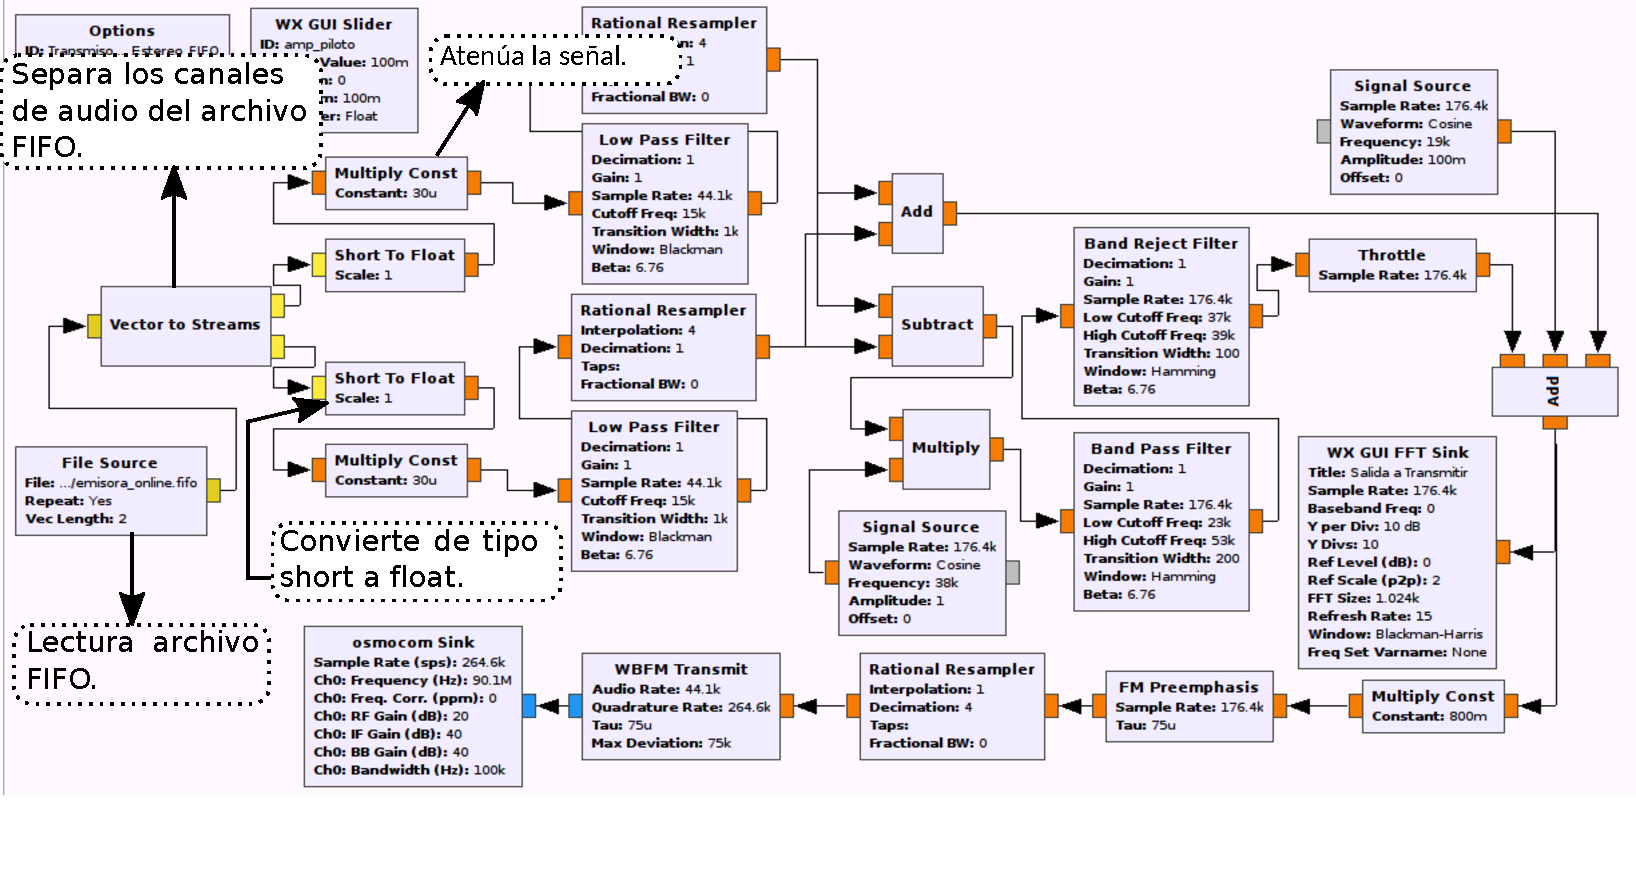
\includegraphics[width=\textwidth]{parte3/lab13/pdf/lab13_3.pdf}
\end{figure}
\end{frame}
%---------------------------------

\begin{frame}{Espectro de señal a transmitir}

\begin{figure}[H]
\centering
\vspace{-3mm}
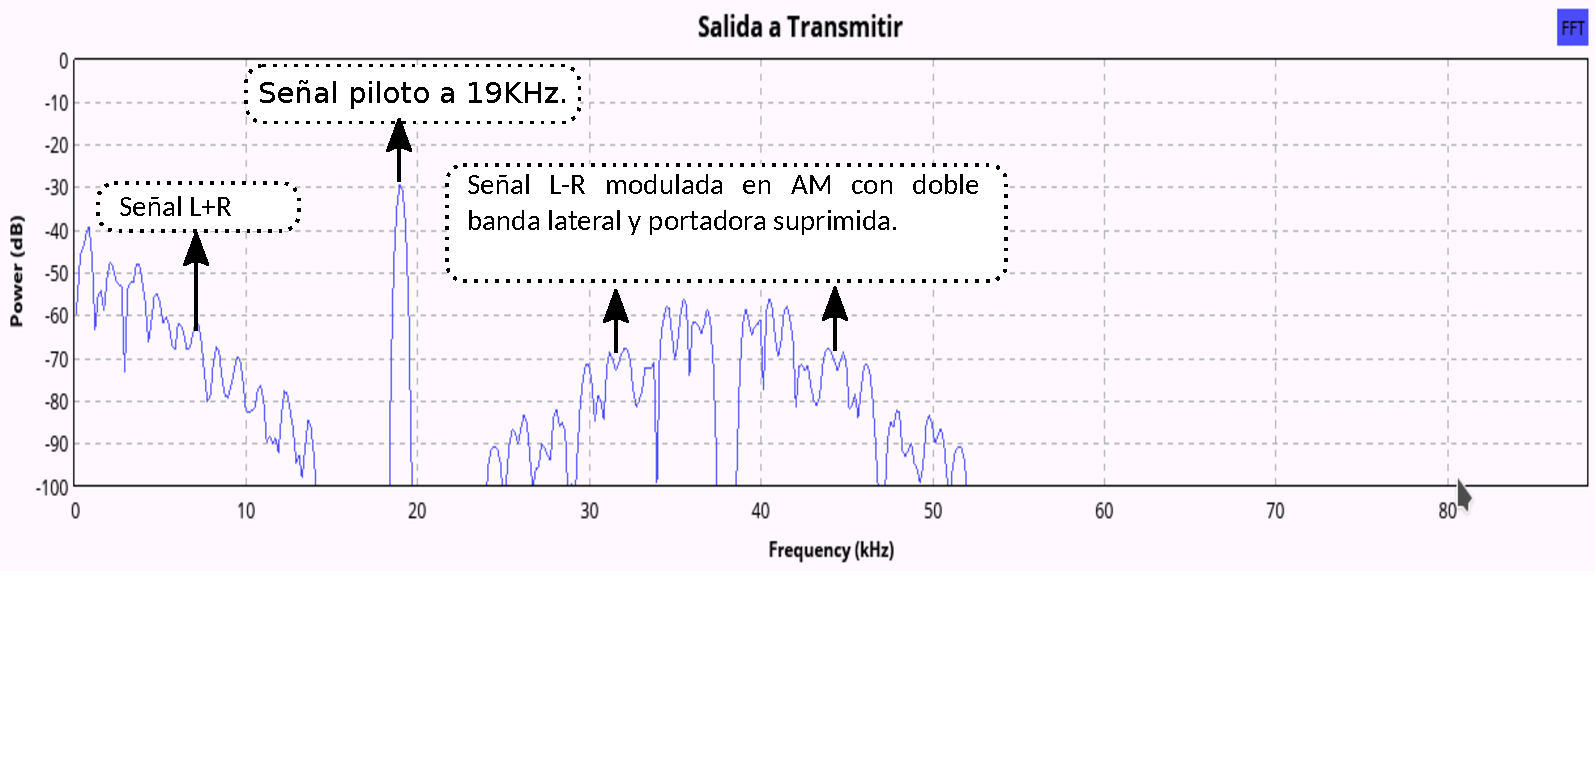
\includegraphics[width=\textwidth]{parte3/lab13/pdf/lab13_4.pdf}
\end{figure}
\end{frame}
%---------------------------------